\documentclass[11pt,twocolumn]{article}
\usepackage{graphicx}
\usepackage{hyperref}
\usepackage{xcolor}
\usepackage{amsmath}
\usepackage{enumitem}
\usepackage{booktabs}
\usepackage{geometry}
\geometry{margin=1in}
\usepackage{placeins}
\usepackage{dblfloatfix}


\title{ZoneWise: Personalized Health Analytics Built on Transparent Retrieval-Augmented Systems}
\author{Mahyar Vahabi \\ University of California, Santa Cruz}
\date{Spring 2026}

\begin{document}

\maketitle

\section{Abstract}
ZoneWise is a full-stack health analytics and conversational intelligence system designed to integrate physiological metrics, personalized user context, and retrieval-augmented generation (RAG) into an engineering architecture designed for future scale. Originally developed as an extension of RootWise, a transparent RAG-based sustainability assistant \cite{faris2025rootwise}, ZoneWise expands the architecture into a production-oriented health platform. 

While RootWise demonstrated transparent retrieval, user-curated knowledge, and modular RAG design, ZoneWise focuses on engineering scalability, data modeling, real-time ingestion, and system performance. The system integrates a FastAPI backend, PostgreSQL data layer, NVIDIA embedding models, FAISS vector indexing, a decoupled agentic reasoning microservice communicating over SSE, and a React-based analytics dashboard. 

This paper emphasizes system design, architectural tradeoffs, and engineering implementation rather than experimental evaluation. ZoneWise demonstrates how transparent RAG systems can evolve into production-oriented, domain-specific health intelligence platforms.

\section{Introduction}

Large language models (LLMs) provide powerful reasoning capabilities but lack persistent personalization, structured metric awareness, and domain-specific reliability. Lily Faris’ RootWise project introduced a transparent Retrieval-Augmented Generation (RAG) architecture to ground LLM responses in curated sustainability data \cite{faris2025rootwise}. RootWise demonstrated:

\begin{itemize}
    \item Transparent document retrieval,
    \item User-controlled knowledge injection,
    \item FAISS-based vector indexing,
    \item Dynamic prompt construction.
\end{itemize}

ZoneWise extends this architecture into a health analytics platform that integrates structured physiological metrics (heart rate, zone durations, recovery metrics) with conversational RAG. Rather than focusing on sustainability and recipe assistance, ZoneWise centers on:

\begin{itemize}
    \item Time-series, metric retrieval,
    \item Mobile-assisted data ingestion
    \item Real-time dashboard visualization,
    \item Personalized zone analysis,
    \item Context-aware health chat grounded in user data.
\end{itemize}

The core contribution of this capstone is the engineering design of a modular health intelligence system built atop transparent RAG principles designed for future scale.

\section{System Overview}

ZoneWise is composed of six primary subsystems:

\begin{enumerate}
    \item Client Interfaces (React dashboard, Android client)
    \item Authentication and API Layer
    \item Structured Data Store (PostgreSQL)
    \item Retrieval-Augmented Intelligence Layer (FAISS + NVIDIA Embeddings)
    \item Conversational Analytics Engine (ZoneWise + RootWise chat)
    \item Agentic Reasoning Service (decoupled SSE microservice)
\end{enumerate}

\begin{figure}[h!]
    \centering
    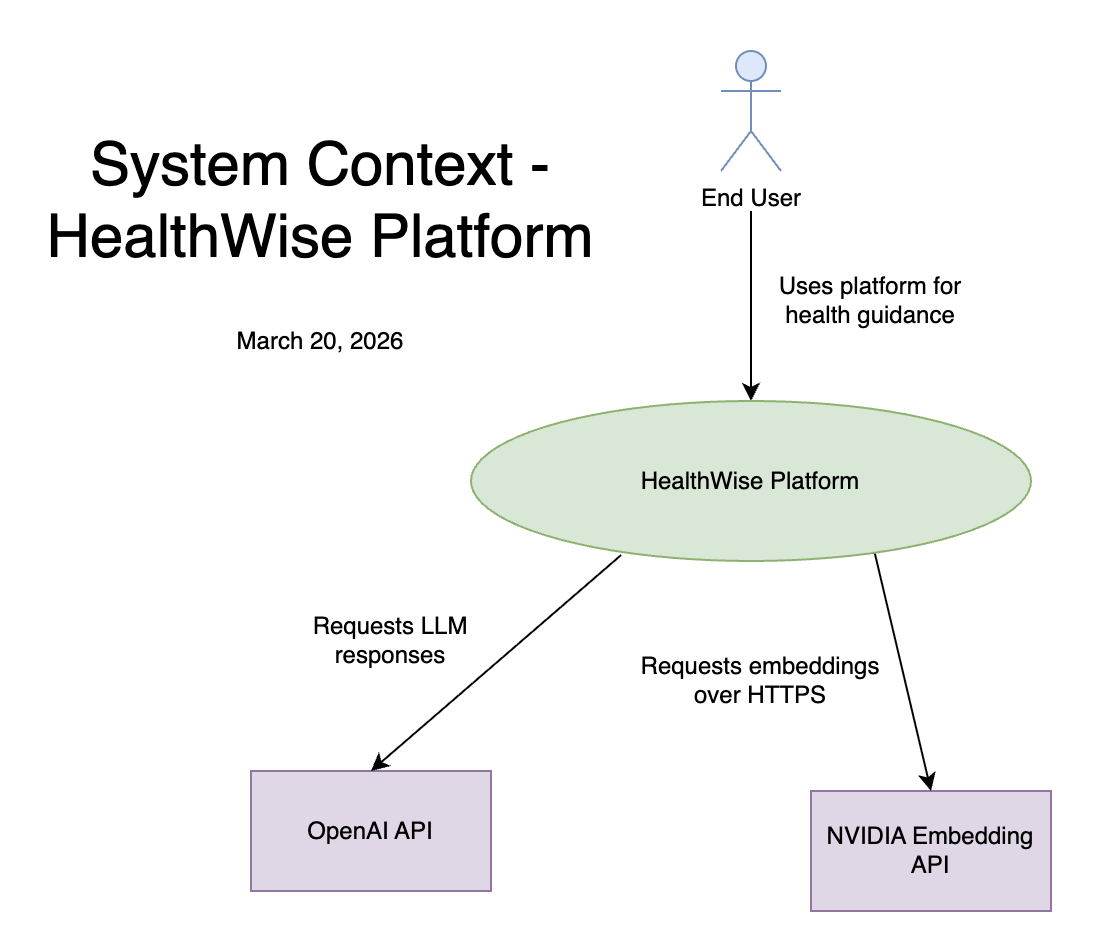
\includegraphics[width=1\linewidth]{SystemContextDiagram.png}
    \caption{System Context Diagram for HealthWise Platform}
    \label{fig:system_context}
\end{figure}



Figure references in RootWise \cite{faris2025rootwise} illustrate the base RAG architecture (embedding model + FAISS + LLM). ZoneWise preserves this pipeline but integrates structured metric awareness.



\section{System Architecture}

\begin{figure}[h!]
    \centering
    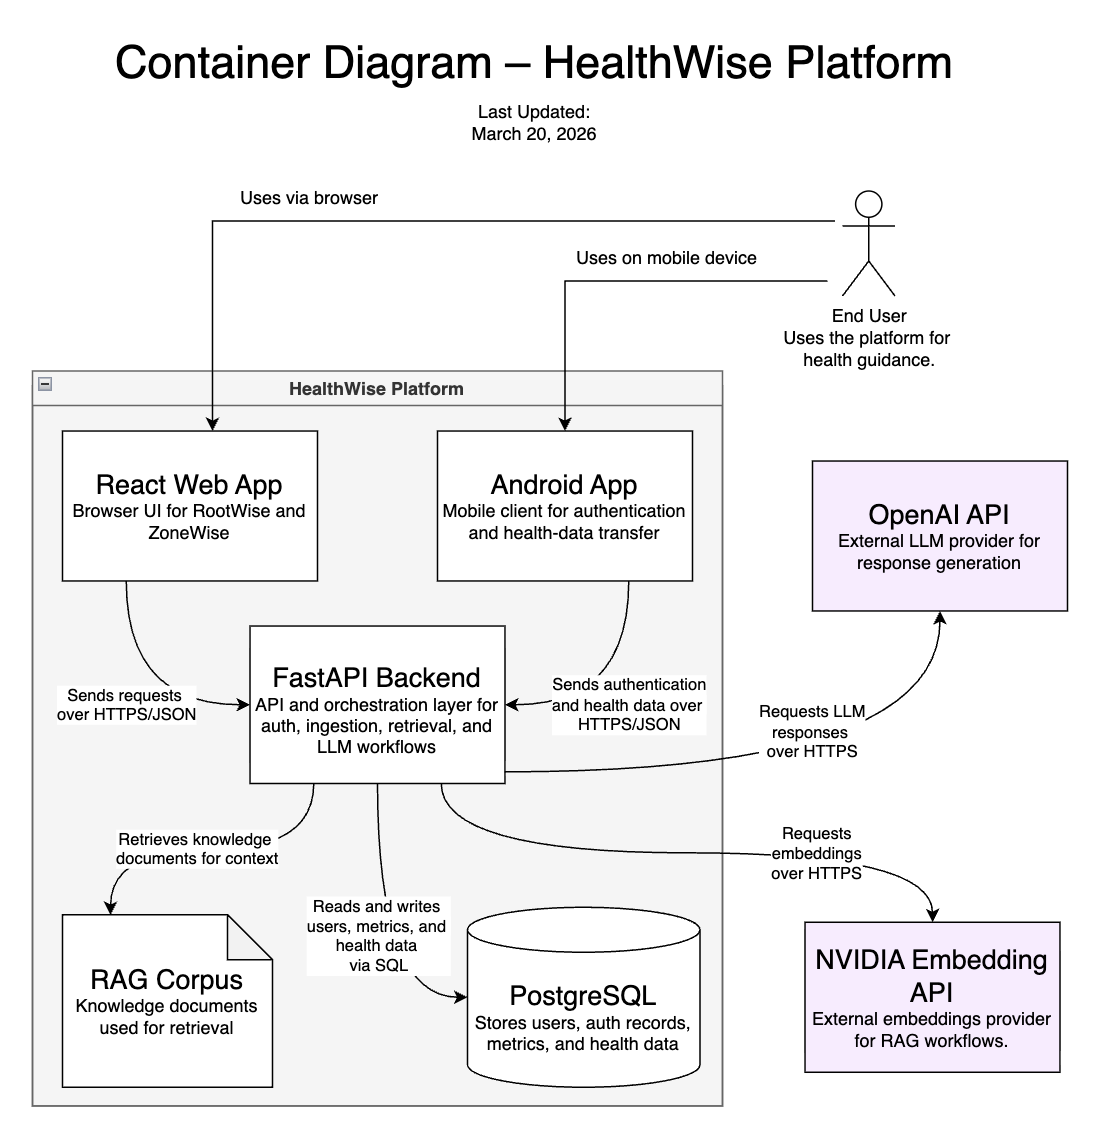
\includegraphics[width=1\linewidth]{ContainerDiagram.png}
    \caption{Container Diagram for HealthWise Platform}
    \label{fig:container}
\end{figure}

ZoneWise follows a modular full-stack architecture designed to separate infrastructure concerns, domain logic, and user interface components. The system consists of a Python FastAPI backend, a PostgreSQL persistence layer, a vector retrieval subsystem for RAG operations, and a React-based frontend. In addition to the browser-based React interface, the broader HealthWise platform also includes a Kotlin-based Android client that can submit authentication and health-related information to the backend. While ZoneWise remains operable through the web application alone, the Android client supplements the platform by streamlining mobile data collection and ingestion. The codebase mirrors this architecture by organizing functionality into distinct backend and frontend modules that correspond directly to system responsibilities.

\subsection{Backend Architecture}

The backend is implemented using FastAPI and structured using a layered architecture. The codebase separates HTTP routing, business logic, and database interaction into dedicated modules, improving maintainability and allowing individual components to evolve independently. The FAISS index is maintained in memory and rebuilt at application startup from the local document corpus. OpenAI API and NVIDIA Embedding API are used as external dependencies.

\begin{figure}[h!]
    \centering
    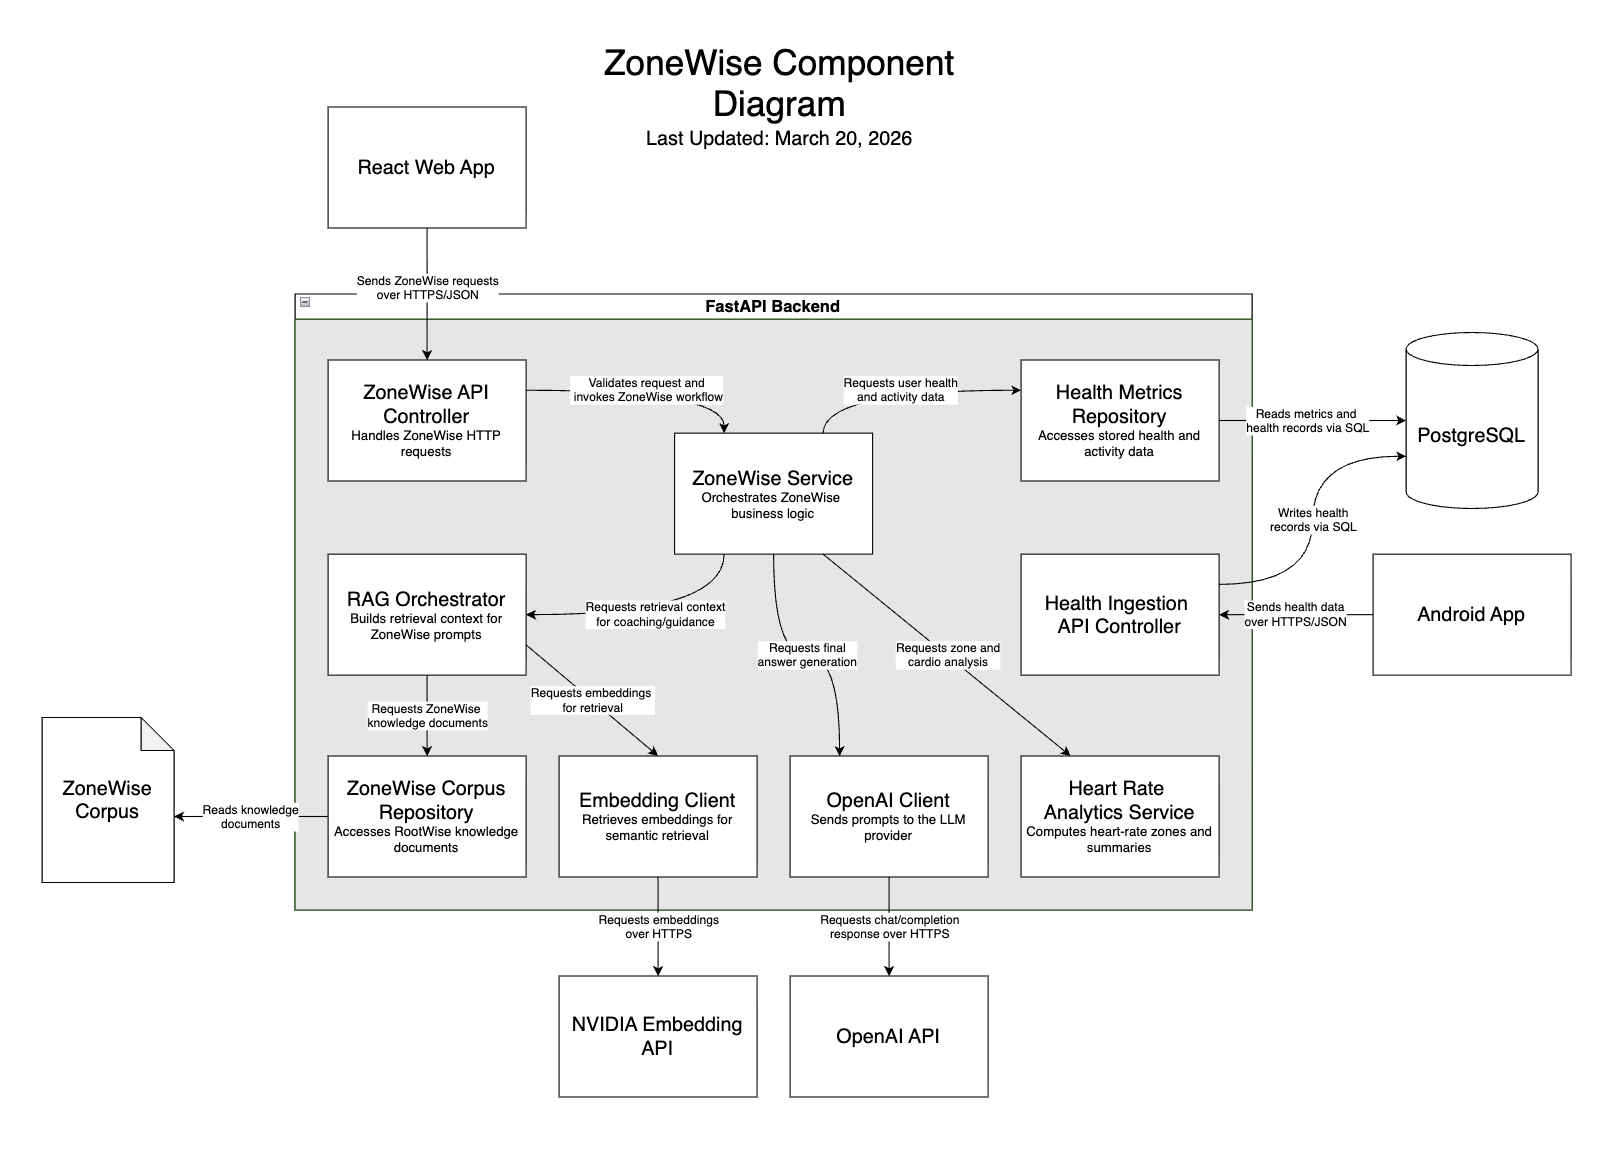
\includegraphics[width=1\linewidth]{ZoneWiseComponentDiagram.png}
    \caption{Component Diagram for ZoneWise}
    \label{fig:zonewise_component}
\end{figure}

At the system level, the backend provides several core services:

\begin{itemize}
    \item REST API endpoints for authentication, metrics, and chat interactions
    \item PostgreSQL data persistence for users and health metrics
    \item JWT-based stateless authentication
    \item Vector retrieval infrastructure using FAISS
    \item Embedding generation using the \texttt{nv-embedqa-e5-v5} model
    \item LLM inference through the OpenAI API
\end{itemize}

These services are implemented through three primary backend modules: \texttt{api}, \texttt{logic}, and \texttt{db}.

\subsubsection{API Layer (\texttt{backend/app/api})}

The API module defines the public REST interface exposed to the frontend. Each route corresponds to a functional capability of the platform such as authentication, metric ingestion, or chat interaction.

Endpoints are implemented using FastAPI routers and use Pydantic models for request validation and response serialization. For example, the authentication router provides the following endpoints:

\begin{itemize}
\item \textbf{/register}: creates a user account and returns a JWT token
\item \textbf{/login}: verifies credentials and generates a session token
\item \textbf{/me}: retrieves authenticated user information
\end{itemize}

Incoming requests are validated before execution, ensuring that user attributes such as age, height, and weight fall within acceptable ranges. Database sessions are injected using FastAPI dependency injection, which ensures safe transaction handling.

\subsubsection{Logic Layer (\texttt{backend/app/logic})}

The logic module encapsulates all domain-level computation independent of HTTP transport. It is subdivided into three functional areas: authentication, the RootWise sustainability assistant, and the ZoneWise health analytics engine. Separating these concerns from the API layer ensures that each domain can evolve independently and be tested without an HTTP server.

\paragraph{Authentication Logic (\texttt{auth.py}, \texttt{auth\_deps.py})}

Authentication logic is implemented using three core operations:

\begin{itemize}
\item password hashing (bcrypt via Passlib)
\item credential verification (constant-time comparison)
\item JWT token creation (HS256 signed, user ID + expiry payload)
\end{itemize}

Authentication enforcement is implemented as reusable FastAPI dependency functions that extract Bearer tokens, validate the JWT payload, and surface the authenticated user identifier to downstream handlers. This enables declarative, stateless security across all protected endpoints.

\paragraph{RootWise Logic (\texttt{logic/rootwise.py})}

\texttt{rootwise.py} implements the full domain logic for the RootWise sustainability and food wisdom assistant. Its responsibilities span four engineering concerns:

\textbf{(1) RAG Index Lifecycle.} A singleton \texttt{RagService} instance is bound to the \texttt{ROOTWISE\_DATA} directory at module load time. \texttt{initialize\_rootwise\_rag()} is called at application startup to build the unified FAISS index over all \texttt{.txt} and \texttt{.pdf} documents in that directory. Index rebuilding is also triggered on document upload via \texttt{load\_documents()}, which copies incoming files into the corpus before re-indexing.

\textbf{(2) User State Management.} User-specific context (current season, on-hand ingredients, dietary restrictions) is persisted as flat text files in \texttt{USER\_STATE\_DIR} via \texttt{add\_to\_rag()}. A named per-user session file (e.g., \texttt{MahyarRAG.txt}) is created via \texttt{set\_user\_name()} and extended by \texttt{append\_to\_user\_rag()}. Critically, this user state is injected into prompts as \emph{constraints}, not as embedded evidence—ensuring it shapes generation without polluting the vector index.

\textbf{(3) Vision Transformer Integration.} \texttt{detect\_vegetables()} spawns \texttt{vis\_transformer.py} as a subprocess to perform image-based ingredient detection. This design isolates the GPU-bound vision model from the main FastAPI process, preventing interference with the async event loop.

\textbf{(4) Grounded Chat with Agentic Query Reformulation.} \texttt{stream\_response()} implements a two-pass agentic retrieval loop. In the first pass, the raw user message is used to retrieve the top-$k$ document chunks from the FAISS index. A hit quality check (\texttt{\_safe\_has\_good\_hits}) evaluates whether at least two retrieved chunks contain substantive text ($>$80 characters). If the initial retrieval is weak, the function invokes the LLM to reformulate the query into a keyword-dense search string and retries retrieval once. If both passes fail, the system declines to answer rather than hallucinate. Successful retrievals are formatted with source attribution and injected into a structured system prompt that enforces inline citation discipline: every factual sentence must end with a bracketed citation \texttt{[n]}, and only citations within the range \texttt{[1..k]} are permitted.

\paragraph{ZoneWise Logic (\texttt{logic/zonewise.py})}

\texttt{zonewise.py} implements the domain logic for the ZoneWise heart-rate zone analytics assistant. Its architecture parallels RootWise but is adapted for physiological metric grounding rather than document-only retrieval.

\textbf{(1) Separate RAG Instance.} ZoneWise maintains its own \texttt{RagService} instance bound to \texttt{ZONEWISE\_DATA}—a separate corpus of heart-rate training science documents. This isolation ensures that zone physiology content does not interfere with the RootWise sustainability index and vice versa.

\textbf{(2) Metric Context Injection.} \texttt{stream\_zonewise\_response()} accepts an optional \texttt{metric\_context} string—a pre-formatted SQL-derived summary of the user's recent physiological measurements (zone durations, heart-rate distributions, time-windowed averages). This structured data is injected into the prompt under a dedicated \texttt{USER\_METRIC\_CONTEXT} block, explicitly separated from the RAG evidence block. The system prompt instructs the model to analyze metric context for personalized trend analysis while citing only from RAG evidence for physiological claims.

\textbf{(3) Structured Response Schema.} The ZoneWise system prompt enforces a rigid five-section output schema: \emph{Summary}, \emph{User Data Insights}, \emph{Document-Grounded Insights} (with mandatory citations), \emph{Recommendations}, and \emph{Confidence}. This schema was designed to separate user-data-derived observations from document-grounded scientific claims, making citation traceability explicit and reducing hallucination risk.

\textbf{(4) Agentic Reformulation Loop.} Identical to RootWise, a weak-hit detector triggers a single LLM-driven query reformulation step before falling back to a graceful refusal. This agentic loop improves recall for queries that are phrased conversationally but map to technical terminology in the corpus.

\textbf{(5) Safety Boundaries.} The system prompt enforces hard constraints: the model must not diagnose medical conditions, must not prescribe medication, and must direct clinical questions to qualified professionals. These boundaries are baked into the system prompt template rather than applied post-hoc, ensuring consistent enforcement across all queries.

\subsubsection{Database Layer (\texttt{backend/app/db})}

The ZoneWise backend uses PostgreSQL as its primary persistence layer, accessed through the SQLAlchemy ORM. The database module is responsible for defining relational models, configuring the database engine, and managing transactional sessions used by API endpoints.

\paragraph{Database Engine and Session Management}

The SQLAlchemy engine is initialized using a database connection string provided through an environment variable (\texttt{DATABASE\_URL}). Environment configuration is loaded using the \texttt{python-dotenv} library, allowing local development and deployment environments to specify database credentials securely.

The engine is created using SQLAlchemy's \texttt{create\_engine} function. A session factory is defined using SQLAlchemy's \texttt{sessionmaker}. Sessions are configured with:

\begin{itemize}
\item \textbf{autocommit=False} to ensure explicit transaction control
\item \textbf{autoflush=False} to prevent unintended writes during query operations
\item \textbf{engine binding} for connection management
\end{itemize}

Each incoming API request obtains a database session through a FastAPI dependency function (\texttt{get\_db}). The dependency yields a session instance that remains active for the duration of the request and is automatically closed after the request completes. This pattern ensures proper resource cleanup and prevents connection leaks.

\paragraph{Database Models}

Persistent entities are represented using SQLAlchemy ORM models located in the \texttt{models} module. Each model corresponds directly to a PostgreSQL table and defines the schema used by the application.

Two primary entities form the core data model:

\begin{center}
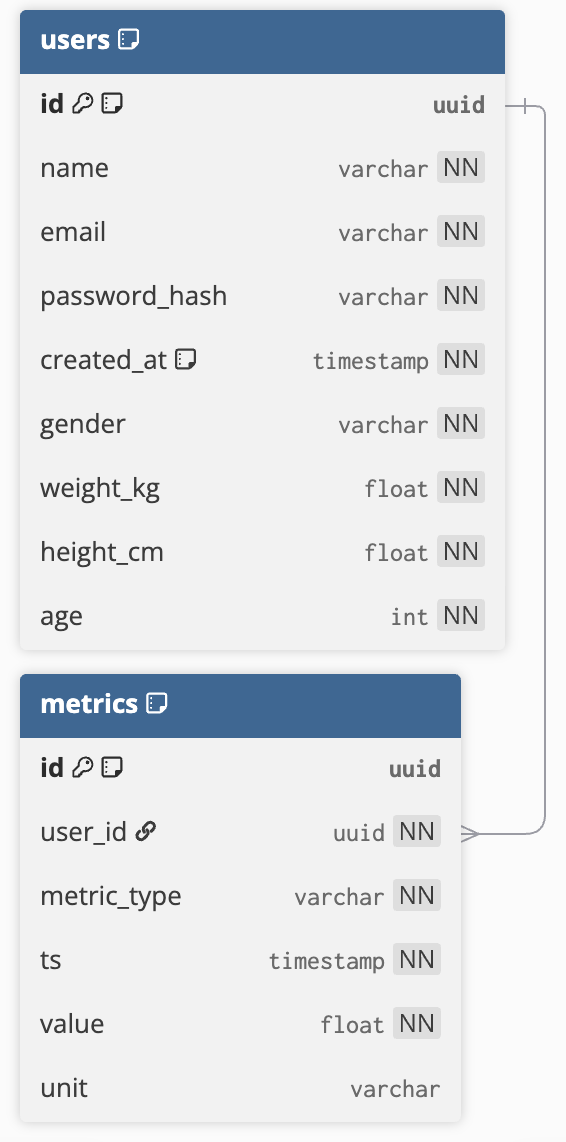
\includegraphics[width=0.3\textwidth]{tables.png}
\end{center}

\begin{itemize}
\item \textbf{User}: stores authentication credentials and demographic attributes such as age, height, and weight.
\item \textbf{Metric}: stores time-series physiological measurements associated with individual users.
\end{itemize}

Metrics reference users through a foreign key relationship, enabling efficient retrieval of historical health data. This schema supports time-window queries used by the analytics dashboard and provides structured context that can be incorporated into RAG prompt construction for personalized health recommendations.


\subsection{Agentic Service Module (\texttt{logic/rootwise\_agentic})}

The \texttt{rootwise\_agentic} package implements a decoupled client for an independently deployed agentic reasoning service. Rather than embedding all agent orchestration logic inside the FastAPI monolith, the architecture delegates advanced multi-step reasoning to a separate process reachable at \texttt{AGENTIC\_SERVICE\_URL}. The main backend communicates with this service via HTTP/SSE streaming, preserving full response visibility without coupling deployment lifecycles.

\subsubsection{Architectural Motivation}

The separation of the agentic service from the main backend is a deliberate architectural decision. Agentic workloads—multi-step tool calls, chain-of-thought reasoning, iterative retrieval loops—have fundamentally different resource profiles and latency characteristics than standard REST handlers. Running them in a separate process allows:

\begin{itemize}
\item Independent horizontal scaling of the reasoning workload
\item Process isolation that protects the main API event loop from blocking operations
\item Independent deployment and versioning of agent logic
\item Transparent observability through trace events emitted over SSE
\end{itemize}

\subsubsection{SSE Transport and Event Protocol}

Communication uses Server-Sent Events (SSE) over an HTTP \texttt{POST} to \texttt{/agentic/chat/stream}. The request payload carries the user's \texttt{message}, prior \texttt{history}, and a \texttt{debug} flag. The response stream emits structured SSE frames, each prefixed with an \texttt{event:} field and a \texttt{data:} JSON payload.

Three event types are defined in \texttt{types.py} as the \texttt{AgenticEvent} TypedDict:

\begin{itemize}
\item \textbf{trace}: Intermediate agent reasoning step. Carries a \texttt{data} payload for diagnostic visibility into agent internals during development.
\item \textbf{message}: Final assistant response. Carries the full updated \texttt{history} list for stateless client-side session management.
\item \textbf{error}: Service-level failure. Triggers a \texttt{RuntimeError} in the calling coroutine with the error detail.
\end{itemize}

\subsubsection{Streaming Client Implementation}

\texttt{service.py} implements the async streaming client using \texttt{httpx.AsyncClient} in streaming mode. The client consumes the raw byte stream in chunks, accumulating them in a buffer and splitting on the double-newline SSE frame delimiter (\texttt{\textbackslash n\textbackslash n}). Each complete SSE frame is passed to \texttt{\_parse\_sse\_chunk()}, which extracts the event name and JSON data, deserializes the payload, and yields a typed \texttt{AgenticEvent} to the caller.

Error handling distinguishes between HTTP status errors (4xx/5xx from the agentic service) and connectivity failures (service unreachable), returning structured error events rather than raising unhandled exceptions. This ensures the main API can always return a well-formed response to the frontend, even when the agentic service is degraded.

\subsubsection{Integration with the API Layer}

The agentic client is invoked from the RootWise API router (\texttt{api/rootwise.py}). The router awaits the async generator and proxies SSE events directly to the frontend, making the full agentic trace visible to clients that opt into debug mode. This architecture creates a transparent three-tier streaming pipeline: frontend $\to$ FastAPI $\to$ agentic service, with event semantics preserved end-to-end.

\subsection{Frontend Architecture}

The frontend is implemented using React and provides the user-facing interface for authentication, health analytics visualization, and conversational interaction. The codebase is organized into modular components that separate API communication, authentication gating, and application views. The React Web App stands as our primary user-facing analytics and chat interface. The Android App provides supplemental health-data contribution client for the broader platform.

\subsubsection{API Communication Layer}

The frontend communicates with the backend through a centralized API client module. This module manages HTTP requests, attaches authentication tokens to requests, and standardizes error handling. 

Authentication tokens are stored in browser local storage and automatically attached to outgoing requests as Bearer tokens. This ensures compatibility with backend JWT authentication dependencies without requiring individual components to manage authentication headers.

A dedicated authentication API module exposes higher-level functions corresponding directly to backend endpoints, including user registration, login, token validation, and logout functionality. These abstractions allow React components to interact with authentication services without directly managing network logic.

\subsubsection{Authentication Gate Component}

The \texttt{AuthGate} component acts as a protective wrapper around authenticated application routes. When the application loads, this component verifies whether a valid JWT token exists and attempts to retrieve the authenticated user's profile from the backend.

If authentication fails, the user is redirected to the login or registration interface. If authentication succeeds, the protected application components are rendered. This pattern ensures that sensitive health data and analytics views are only accessible to authenticated users.

\subsubsection{Main Application View}

The \texttt{ZoneWise.jsx} component functions as the primary application dashboard. It coordinates several frontend features including:

\begin{itemize}
\item user authentication state management
\item health metric visualization
\item chat-based interaction with the RAG assistant
\end{itemize}

The component maintains application state such as user profile information, authentication status, and recent metric data. It also integrates charting libraries for displaying zone-based health metrics and time-series analytics derived from the backend database.

By centralizing these functions, \texttt{ZoneWise.jsx} acts as the orchestration layer for the client-side application.

\subsubsection{Chat Interface Component}

The conversational interface is implemented through the \texttt{Chat.jsx} component. This component manages the lifecycle of user interactions with the ZoneWise conversational assistant.

Key responsibilities include:

\begin{itemize}
\item maintaining the chat message history
\item sending user queries to the backend chat endpoint
\item streaming assistant responses to the interface
\item automatically scrolling and updating the conversation view
\end{itemize}

When a user submits a message, the component sends the request to the backend chat streaming endpoint:

\texttt{/api/zonewise/chat/stream}


The backend retrieves relevant user metrics and RAG context before generating a response from the language model. The response is streamed back to the frontend and appended to the conversation history in real time.

\subsection{End-to-End Authentication Flow}

The complete authentication workflow proceeds as follows:

\begin{enumerate}
\item A user submits login or registration credentials through the React interface.
\item The frontend sends a request to the backend authentication API.
\item The backend verifies credentials and generates a signed JWT token.
\item The token is stored in browser local storage.
\item Future API requests automatically include the token in the Authorization header.
\item Backend authentication dependencies validate the token and extract the user identifier.
\item Protected endpoints retrieve user-specific metrics and health data.
\end{enumerate}

Because authentication is stateless, the backend can scale horizontally without maintaining server-side sessions.

\subsection{Architectural Benefits}

The ZoneWise architecture tightly integrates system design with code organization. Backend modules encapsulate authentication, data persistence, and AI-driven processing, while frontend components manage user interaction and visualization.

This modular design enables the platform to scale as additional features such as expanded metric ingestion pipelines, advanced analytics, or improved RAG-based health recommendations are introduced.


\section{Personalized RAG Architecture}

The ZoneWise RAG pipeline is a hybrid retrieval system that merges two orthogonal retrieval modalities: deterministic SQL queries over structured physiological data, and probabilistic semantic search over a curated health guidance corpus.

\subsection{Dual-Source Retrieval Design}

\textbf{Structured retrieval} is performed via SQLAlchemy queries against the \texttt{Metric} table. The backend computes time-windowed aggregations over configurable lookback windows (30, 60, and 90 days) to produce per-user summaries of zone distribution, heart-rate averages, and training volume. This data is serialized into a formatted \texttt{metric\_context} string before being passed into the RAG pipeline.

\textbf{Semantic retrieval} is performed by \texttt{RagService}, which maintains a per-corpus FAISS \texttt{IndexFlatL2} index built from sentence-split chunks of curated \texttt{.txt}/\texttt{.pdf} documents. Queries are embedded using the \texttt{nvidia/nv-embedqa-e5-v5} model (accessed via the NVIDIA NGC API) and matched against stored document embeddings using exact $L_2$ distance, returning the top-$k$ most similar chunks.

\subsection{Prompt Construction Pipeline}

Prompt assembly follows a strict separation-of-concerns principle inherited from RootWise \cite{faris2025rootwise}. The final prompt passed to the LLM contains three distinct blocks:

\begin{enumerate}
    \item \textbf{USER\_METRIC\_CONTEXT}: SQL-derived physiological summary (no citations permitted)
    \item \textbf{EVIDENCE}: FAISS-retrieved document chunks with source and page metadata (all factual claims must cite from this block)
    \item \textbf{USER QUESTION}: The raw user query
\end{enumerate}

This architecture makes retrieval transparent: the model cannot blend user-data observations with document-grounded claims because the system prompt prohibits citing \texttt{USER\_METRIC\_CONTEXT} and mandates that every physiological claim carries a bracketed evidence citation.

\subsection{Agentic Retrieval Loop}

Both ZoneWise and RootWise implement a single-iteration agentic retrieval fallback. When the hit quality check—requiring at least two chunks with $>$80 characters of substantive text—fails on the initial query, the system makes a secondary LLM call to reformulate the query into a keyword-dense search string before retrying. This loop improves recall for colloquial or vague queries while avoiding unbounded recursion. If both retrieval passes fail, the system returns a transparent refusal rather than generating unsupported content.

\section{Streaming Chat Architecture}

The platform exposes two streaming chat endpoints, each backed by a different intelligence pipeline:

\begin{verbatim}
POST /api/zonewise/chat/stream
POST /api/rootwise/agentic/chat/stream
\end{verbatim}

\subsection{ZoneWise Chat Pipeline}

The ZoneWise streaming endpoint executes the following pipeline per request:

\begin{enumerate}
    \item Authenticate the request via JWT dependency injection
    \item Query PostgreSQL for the authenticated user's time-windowed metric history and serialize into \texttt{metric\_context}
    \item Invoke \texttt{stream\_zonewise\_response()} with the user message, session history, and \texttt{metric\_context}
    \item Execute the FAISS semantic retrieval pass (with optional agentic reformulation fallback)
    \item Assemble the three-block prompt (metrics + evidence + question)
    \item Submit to the OpenAI Chat Completions API and stream the token output back to the client as newline-delimited JSON
\end{enumerate}

The structured response schema (Summary / User Data Insights / Document-Grounded Insights / Recommendations / Confidence) is enforced by the system prompt, not post-processed, keeping generation latency low.

\subsection{RootWise Agentic Chat Pipeline}

The RootWise agentic endpoint proxies requests through the decoupled agentic service rather than executing inference inline. The FastAPI handler passes the message and history to \texttt{stream\_agentic\_response()}, which opens an \texttt{httpx} streaming connection to the agentic service and relays SSE frames to the frontend verbatim. This three-tier streaming chain—frontend $\to$ FastAPI $\to$ agentic service—allows the agentic service to emit intermediate trace events that the frontend can render as step-by-step reasoning visibility, consistent with the transparent RAG philosophy of RootWise \cite{faris2025rootwise}.

\subsection{Latency Profile}

LLM inference dominates end-to-end latency in both pipelines. FAISS retrieval is sub-millisecond at current corpus sizes. The primary optimization applied is prompt token budgeting: the evidence formatter caps each retrieved chunk at 900 characters, and chat history is truncated to the two most recent turns (300 characters each) before prompt assembly.

\section{Engineering Tradeoffs}

In the current implementation, the FAISS index is maintained in memory and rebuilt at application startup from the local document corpus. This design simplifies development and avoids index synchronization complexity, but increases startup cost and limits persistence across restarts.

\subsection{Vector Store Design}

Current implementation uses \texttt{IndexFlatL2}. Tradeoffs:

\begin{itemize}
    \item Exact search: high accuracy
    \item Poor scaling beyond large corpora
\end{itemize}

Future work includes IVF or HNSW indexing.

\subsection{Latency vs Accuracy}

LLM calls dominate latency. Mitigations:

\begin{itemize}
    \item Prompt compression
    \item Context window pruning
    \item Metric caching
\end{itemize}

\subsection{Structured vs Semantic Retrieval}

ZoneWise blends:

\begin{itemize}
    \item Deterministic SQL filtering
    \item Probabilistic semantic retrieval
\end{itemize}

This reduces hallucination risk relative to pure RAG.

\section{Scalability Considerations}

\begin{itemize}
    \item Horizontal scaling via containerization
    \item Read-replica PostgreSQL
    \item Distributed Celery workers
    \item GPU-backed embedding services
\end{itemize}

\section{Security and Authentication}

\begin{itemize}
    \item JWT-based authentication
    \item Hashed passwords (bcrypt)
    \item Role-based endpoint restriction
    \item Secure environment variable management
\end{itemize}

\section{Comparison with RootWise}

RootWise \cite{faris2025rootwise} focused on:

\begin{itemize}
    \item Sustainable food guidance
    \item Image-based ingredient detection
    \item Transparent RAG
\end{itemize}

ZoneWise extends the architecture by:

\begin{itemize}
    \item Introducing structured metric ingestion
    \item Building a production-oriented backend
    \item Integrating time-series analytics
    \item Supporting real-time streaming chat
\end{itemize}

RootWise primarily grounded qualitative sustainability/nutrition assistance in retrieved documents and demonstrated feasibility of transparent RAG.\\
ZoneWise combines retrieved health guidance with structured physiological data and computations and demonstrates engineering maturation into an analytics platform designed for future scale.


\section{Conclusion}

ZoneWise transforms transparent RAG principles into a production-oriented health analytics system. By combining:

\begin{itemize}
    \item Structured metric storage,
    \item API-based health data ingestion,
    \item Hybrid SQL + vector retrieval,
    \item Real-time conversational intelligence,
\end{itemize}

the system demonstrates how retrieval-augmented AI can evolve from a prototype assistant into a full-stack personalized analytics platform.

Future work includes:

\begin{itemize}
    \item Hardware acceleration,
    \item Smarter vector indexing,
    \item Adaptive metric summarization,
    \item Deployment to distributed cloud infrastructure.
\end{itemize}

ZoneWise illustrates the architectural path from transparent AI prototype to modular engineering system designed for future scale.



\section*{Acknowledgements}

The authors would like to thank Lily Faris for her work on the RootWise project and for allowing this project to build upon and extend the original system. The ZoneWise platform was developed by extending and modifying portions of the RootWise codebase, adapting its transparent Retrieval-Augmented Generation (RAG) architecture to support personalized health analytics and physiological data integration.

The authors also thank Fariha Lateef for her assistance in gathering the medical and functional health reference materials used to initialize the knowledge base for both the RootWise and ZoneWise RAG systems. These curated medical and nutrition documents served as foundational sources for the retrieval pipeline and significantly contributed to the domain grounding of the assistant.

Their contributions were instrumental in enabling the development and expansion of the ZoneWise platform.

\begin{thebibliography}{9}

\bibitem{faris2025rootwise}
Lily Faris.
\textit{RootWise: Utilizing RAG AI for Food Wisdom and Zero-Waste Action}.
University of California, Santa Cruz, 2025.
Available at: \url{https://lilymfaris.com/cappaper.pdf}
\cite{faris2025rootwise}



\end{thebibliography}

\end{document}